% ******************************************************** %
%              TEMPLATE DE INFORME ORGA2 v0.1              %
% ******************************************************** %
% ******************************************************** %
%                                                          %
% ALGUNOS PAQUETES REQUERIDOS (EN UBUNTU):                 %
% ========================================t
%                                                          %
% texlive-latex-base                                       %
% texlive-latex-recommended                                %
% texlive-fonts-recommended                                %
% texlive-latex-extra?                                     %
% texlive-lang-spanish (en ubuntu 13.10)                   %
% ******************************************************** %


\documentclass[a4paper]{article}
\usepackage[spanish]{babel}
\usepackage[utf8]{inputenc}
\usepackage{charter}   % tipografia
\usepackage[pdftex]{graphicx}
\usepackage{graphicx}

\graphicspath{{../codigo/experimentacion/}}
%\usepackage{makeidx}
\usepackage{paralist} %itemize inline
\usepackage{multirow}
\usepackage{graphicx}
\usepackage[table,xcdraw]{xcolor}


\usepackage{float}
\usepackage{amsmath, amsthm, amssymb}
%\usepackage{amsfonts}
%\usepackage{sectsty}
%\usepackage{charter}
%\usepackage{wrapfig}
%\usepackage{listings}
%\lstset{language=C}

% \setcounter{secnumdepth}{2}
\usepackage{underscore}
\usepackage{caratula}
\usepackage{url}
\usepackage{multicol}

% ********************************************************* %
% ~~~~~~~~              Code snippets             ~~~~~~~~~ %
% ********************************************************* %

\usepackage{color} % para snipets de codigo coloreados
\usepackage{fancybox}  % para el sbox de los snipets de codigo

\definecolor{litegrey}{gray}{0.94}
\definecolor{white}{RGB}{255,255,255}

\newenvironment{codesnippet}{%
	\begin{Sbox}\begin{minipage}{\textwidth}\sffamily\small}%
	{\end{minipage}\end{Sbox}%
		\begin{center}%
		\vspace{-0.4cm}\colorbox{litegrey}{\TheSbox}\end{center}\vspace{0.3cm}}



% ********************************************************* %
% ~~~~~~~~         Formato de las páginas         ~~~~~~~~~ %
% ********************************************************* %

\usepackage{fancyhdr}
\pagestyle{fancy}

%\renewcommand{\chaptermark}[1]{\markboth{#1}{}}
\renewcommand{\sectionmark}[1]{\markright{\thesection\ - #1}}

\fancyhf{}

\fancyhead[LO]{Sección \rightmark} % \thesection\ 
\fancyfoot[LO]{\small{Facundo Linlaud, Marco Sotomayor}}
\fancyfoot[RO]{\thepage}
\renewcommand{\headrulewidth}{0.5pt}
\renewcommand{\footrulewidth}{0.5pt}
\setlength{\hoffset}{-0.8in}
\setlength{\textwidth}{16cm}
%\setlength{\hoffset}{-1.1cm}
%\setlength{\textwidth}{16cm}
\setlength{\headsep}{0.5cm}
\setlength{\textheight}{25cm}
\setlength{\voffset}{-0.7in}
\setlength{\headwidth}{\textwidth}
\setlength{\headheight}{13.1pt}

\renewcommand{\baselinestretch}{1.1}  % line spacing

\usepackage{xspace}
\newcommand{\Alpha}{\ensuremath{\mathsf{a}}\xspace}
\newcommand{\Red  }{\ensuremath{\mathsf{r}}\xspace}
\newcommand{\Green}{\ensuremath{\mathsf{g}}\xspace}
\newcommand{\Blue }{\ensuremath{\mathsf{b}}\xspace}

% ******************************************************** %


\begin{document}


\thispagestyle{empty}
\materia{Probabilidad y Estadística}
\submateria{Primer Cuatrimestre de 2019}
\titulo{Trabajo Práctico II}
% \subtitulo{}
\integrante{Facundo Linlaud}{561/16}{facundolinlaud@gmail.com}
\integrante{Marco Sotomayor}{?}{marco.soto1995@gmail.com}

\maketitle
\newpage
%_________________________________________________________________________________________________________________

\thispagestyle{empty}
\vspace{3cm}
\tableofcontents
\newpage

%\normalsize
\newpage

\section{Estimaciones del parámetro b}
\subsection{Método de momentos}
Planteemos el momento muestral de primer orden:

\begin{align*}
	&E(X) = \frac{\sum_{i=1}^{n}X_{i}}{n} \\
\end{align*}

Como $X_{1}, \dots, X_{n}$ es una muestra aleatoria de una distribución $U[0, b]$, podemos igualar el primer momento muestral a la esperanza de la distribución con parámetros $0$ y $b$:

\begin{align*}
	\frac{\sum_{i=1}^{n}X_{i}}{n} = E(X) &\implies \\
	\frac{\sum_{i=1}^{n}X_{i}}{n} = \frac{b}{2} &\implies \\
	\bar{X} = \frac{b}{2} &\implies \\
	2 \cdot \bar{X} = b&
\end{align*}

De esta manera, obtenemos la expresión del estimador del parámetro $b$:

\begin{align*}
	\hat{b}_{mom} = 2 \bar{X}_{n}
\end{align*}

\subsection{Estimador de Máxima Verosimilitud}
Sabemos que la función de densidad de una distribución uniforme es:
$$f_{X}(x)=\frac{1}{b - a}I_{(a, b)}(x)$$
Sabiendo que $a = 0$ y que $a < b$ por propiedades de distribución uniforme, procederemos a maximizar $f_{X}(x)$ para estimar el valor de máxima verosimilitud de $b$:

\begin{align*}
	L(b) &= \prod_{i=1}^{n}\frac{1}{b - a}I_{(a, b)}(x) \\
	\iff L(b) &= \prod_{i=1}^{n}\frac{1}{b - 0}I_{(a, b)}(x) \\
	\iff L(b) &= \prod_{i=1}^{n}\frac{1}{b}I_{(x_{i}, +\infty)}(b)
\end{align*}

Por lo tanto:

\begin{center}
\begin{displaymath}
L(b) = \left\{
\begin{array}{l l}
			\frac{1}{b^n} & \text{si }max\{x_{1}, \dots, x_{n}\} < b\\
			0 & \text{sino}
\end{array}
\right.
\end{displaymath}
\end{center}

Esto implica que $\frac{1}{b^n}$ es máximo cuando $b^n$ es mínimo. Luego, el valor más chico posible de $b$ es el valor más grande que haya tomado algún resultado en la muestra $X_{1}, \dots, X_{n}$. Porque si $b$ fuese menor a alguno de ellos, la probabilidad total sería nula (por contener un elemento fuera del rango de la distribución). Finalmente, tenemos un valor para nuestro estimador:
$$\hat{b}_{mv} = max\{x_{1}, \dots, x_{n}\}$$
\section{Ejercicio 2}
Dada una muestra $X_{1}, ..., X_{n}$, estimar el doble de su mediana implica tomar los únicos datos que tenemos, es decir la muestra, calcular su mediana muestral y multiplicarla por dos. Su implementación puede ser observada en el archivo \textbf{tp2.py}.
\section{Valores y errores de los estimadores para muestra de tamaño 15}
Con una muestra aleatoria de tamaño 15 de una distrubición uniforme con parámetros $[0, 2]$, calculamos los estimadores correspondientes y sus errores. Este último paso es realizado restando el estimador por el valor real del parámetro que el estimador intenta justamente aproximar. Los resultados son:

\begin{table}[H]
	\centering
	\begin{tabular}{lccc}
		\textbf{Estimador} 	&	Valor 		& Error 	\\
		$\hat{b}_{mv}$  	&	0.838 		& $0.161$ 	\\
		$\hat{b}_{mom}$     &	0.920 		& $0.079$ 	\\
		$\hat{b}_{med}$  	&	1.135 		& $-0.135$
	\end{tabular}
\end{table}
\section{Ejercicio 4}
Ver \textbf{tp2.py}.
\section{Ejercicio 5}

\begin{figure}[H]
	\centering
	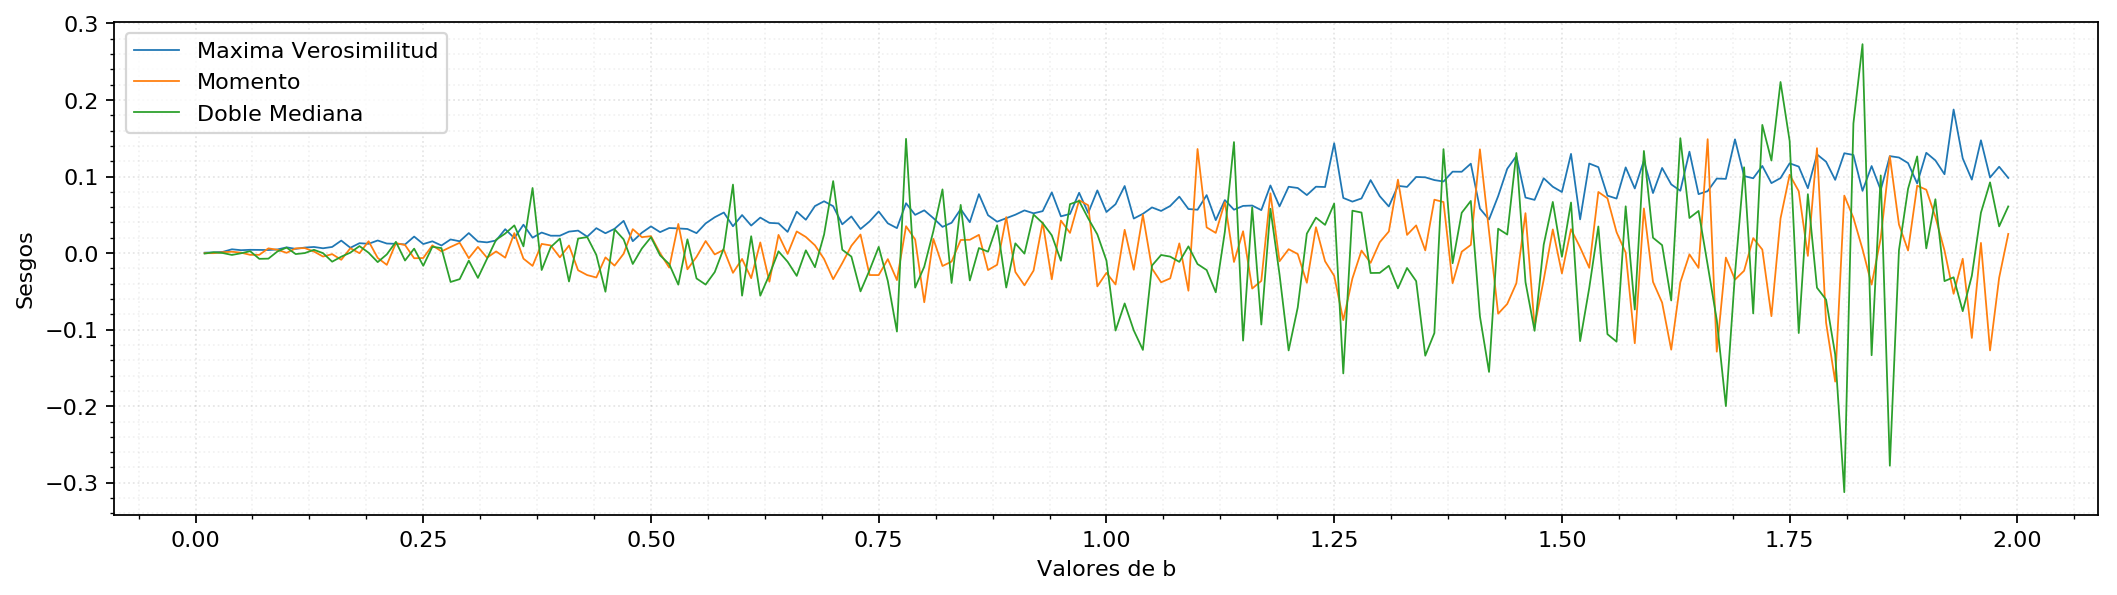
\includegraphics[width=1\textwidth]{imagenes/sesgos.png}
	\caption{\footnotesize Footnotesize}
	% \label{fig:gr-M-n101-k10-K-1-to-30}
\end{figure}

\begin{figure}[H]
	\centering
	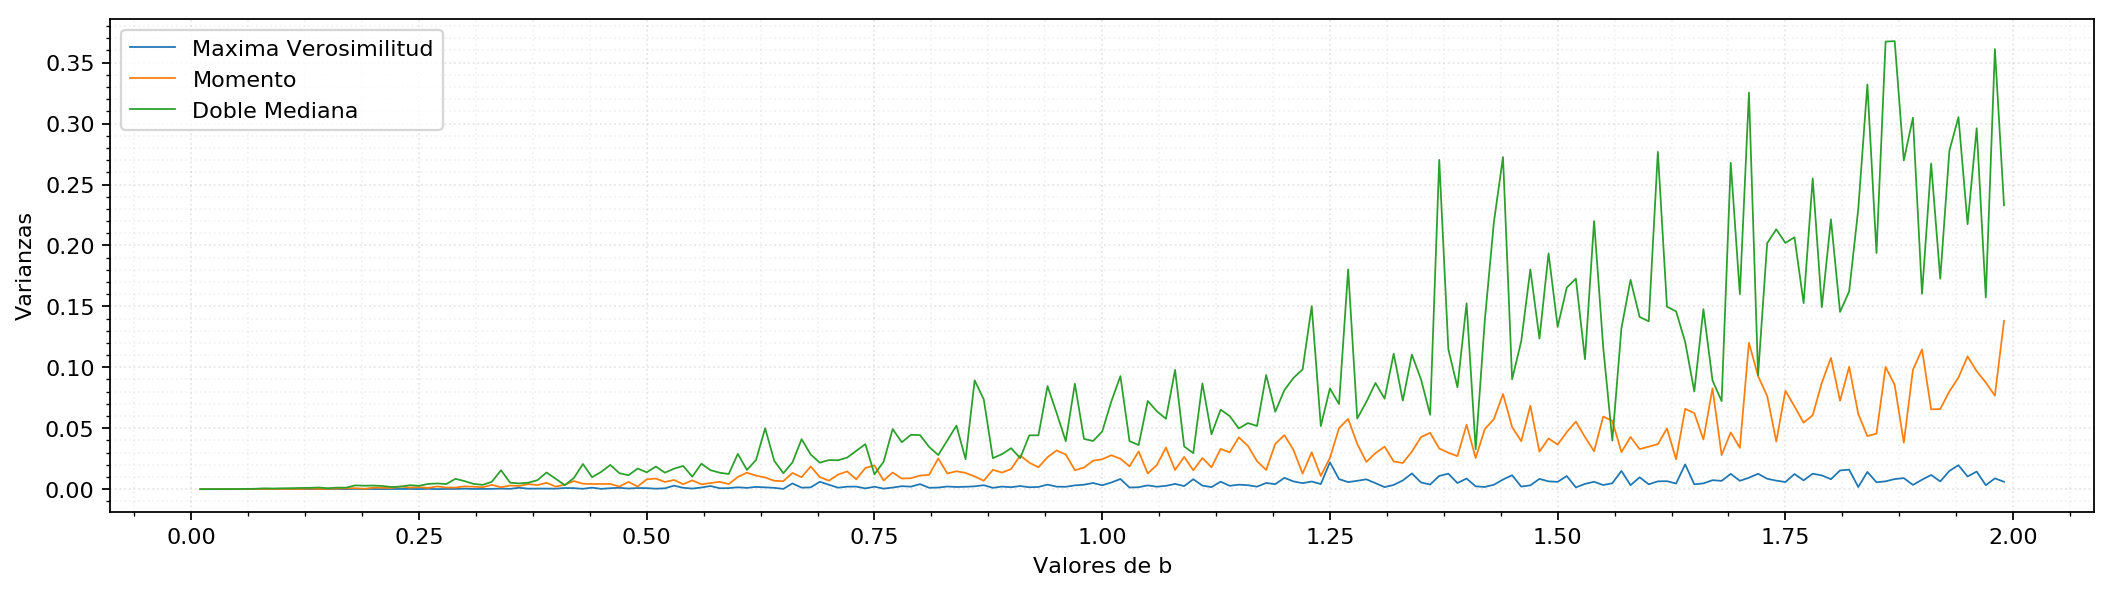
\includegraphics[width=1\textwidth]{imagenes/varianzas.png}
	\caption{\footnotesize Footnotesize}
	% \label{fig:gr-M-n101-k10-K-1-to-30}
\end{figure}

\begin{figure}[H]
	\centering
	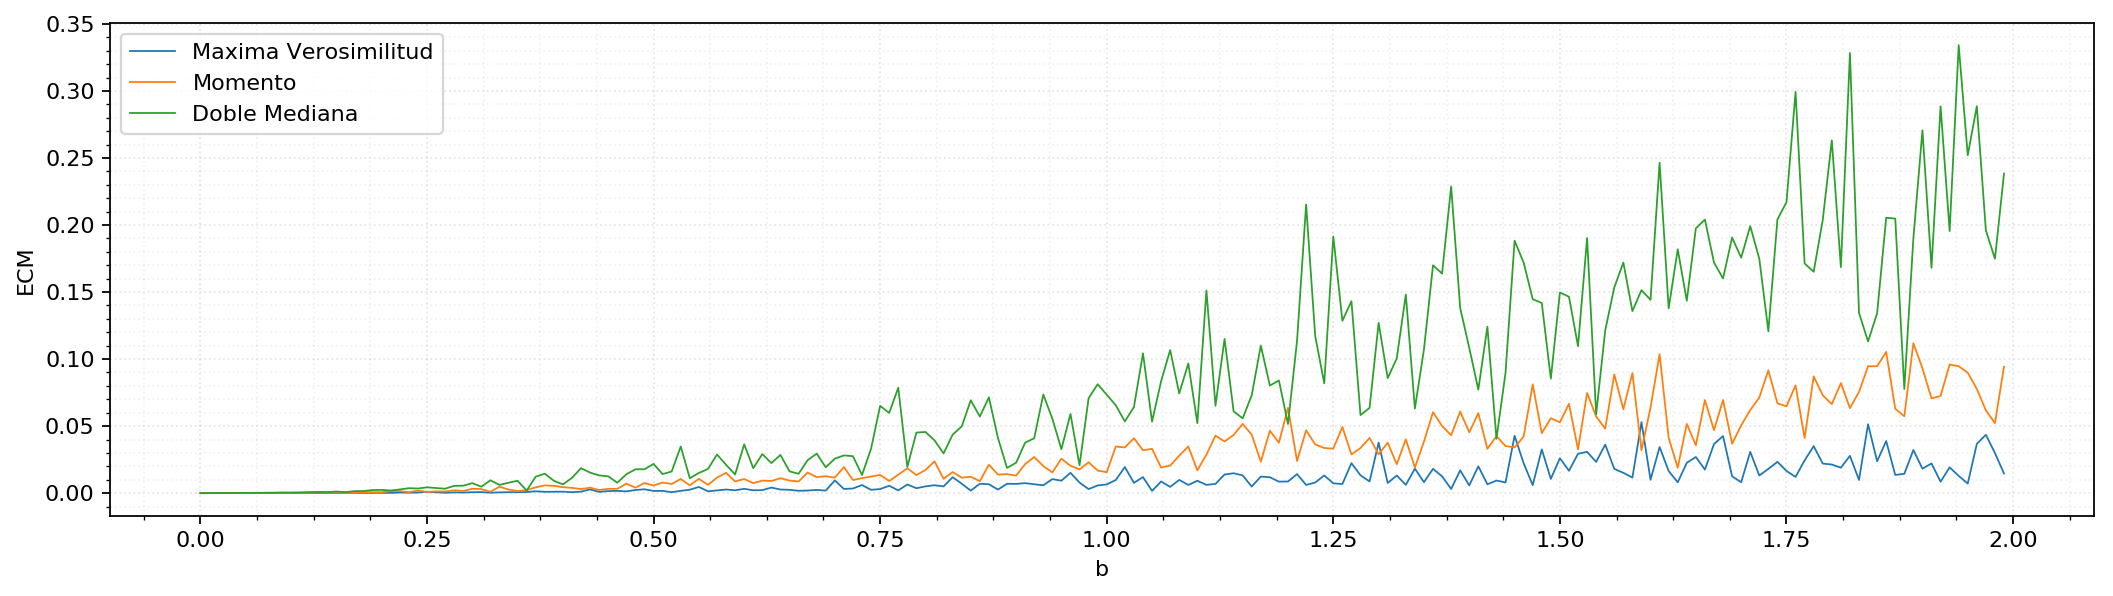
\includegraphics[width=1\textwidth]{imagenes/ecm.png}
	\caption{\footnotesize Footnotesize}
	% \label{fig:gr-M-n101-k10-K-1-to-30}
\end{figure}

\end{document}

